\documentclass{standalone}
\usepackage{pgfplots}
\pgfplotsset{compat=newest}

\begin{document}
	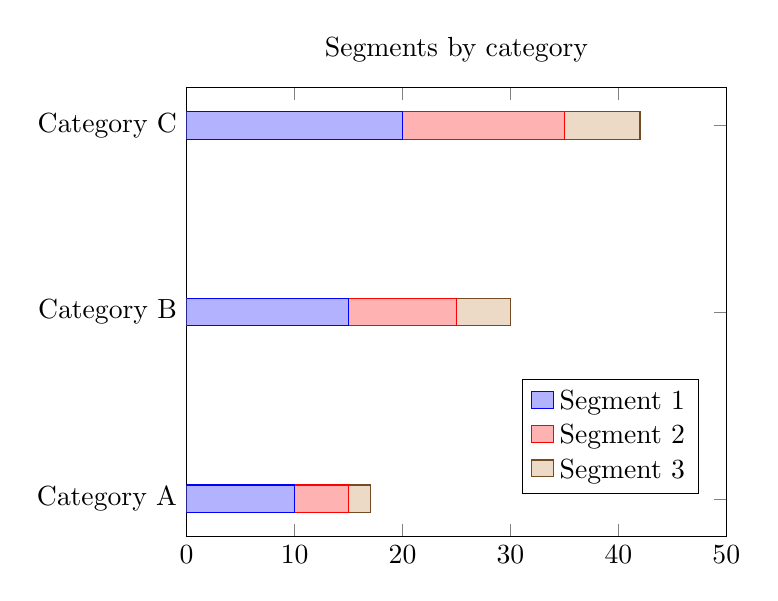
\begin{tikzpicture}
		\begin{axis}[
			xbar stacked, 
			title=Segments by category,
			symbolic y coords={Category A, Category B, Category C},
			ytick=data,			
			legend style={
				at={
					(0.95, 0.35)
				}
			},
			xmin=0,
			xmax=50]
			\addplot plot coordinates {
				(10,Category A)
				(15,Category B)
				(20,Category C)
			};
			
			\addplot plot coordinates {
				(5,Category A)
				(10,Category B)
				(15,Category C)
			};
			
			\addplot plot coordinates {
				(2,Category A)
				(5,Category B)
				(7,Category C)
			};
			
			\legend{Segment 1, Segment 2, Segment 3}
		\end{axis}
	\end{tikzpicture}
\end{document}
